
%\documentclass[12pt]{amsart}
%\usepackage{geometry} % see geometry.pdf on how to lay out the page. There's lots.
%\usepackage{datetime}
%\usepackage{setspace}
%\doublespacing
%\geometry{a4paper} % or letter or a5paper or ... etc
%% \geometry{landscape} % rotated page geometry
%
%% See the ``Article customise'' template for come common customisations
%
%\title{Wind chapter}
%\author{Percy Link}
%\date{\currenttime \ \today} % delete this line to display the current date
%
%%%% BEGIN DOCUMENT
%\begin{document}
%
%\maketitle

\section{Methods}

The sensitivity of Solano wind forecasts to soil moisture is tested using experiments with a regional atmospheric model, the Weather Research and Forecasting (WRF) model.  The WRF model, described in detail in Skamarock et al. [2008], is a three-dimensional, non-hydrostatic regional atmospheric model with terrain-following vertical coordinates.  WRF solves the discretized equations for conservation of momentum, mass, energy, and scalars like water vapor, and it has a range of parameterization options for radiation, turbulence treatment via planetary boundary layer (PBL) schemes or large-eddy simulation closures, cloud microphysics, convection, bottom boundary fluxes of water vapor and heat, and lateral boundary forcing.  WRF has been used extensively in wind energy forecasting [CITATIONS], with generally good performance [CITATIONS].  Accuracy of WRF-forecasted turbine-level winds depends on \textit{(resolution, PBL scheme, lateral forcing, soil moisture **)} [CITATIONS].

\subsection{Model setup}

We run WRF with two nested domains centered on the Solano wind farm (Figure \ref{fig:windSol_domainmap}); the domains are described in Table \ref{table:windSol_domains}.  The use of two nests enables gradual down-scaling of the coarse lateral forcing to the high resolution needed to resolve flow over the Solano wind farm.  We adopt a conservative nesting grid ratio of 3:1; the outer grid forces the lateral boundaries of the inner grid, and the inner grid feeds back to the outer grid across the region where the two domains coincide [Skamarock et al., 2008].  The inner domain has a horizontal resolution of 2.7 km; preliminary tests with a third finer grid (0.9 km) showed little change in the forecasted winds, similar to the results of Marjanovic \textit{et al.} [2014], who found little accuracy improvement with horizontal resolution below 2.7 km in their simple terrain case.  The domain has 45 vertical levels, with a minimum spacing of $\sim$30 m near the surface and a maximum spacing of \textbf{XX at the top of the model domain}, interpolated quadratically by the log of pressure (the default WRF setting); turbine-level (60-100 m) wind forecasts are not very sensitive to vertical resolution beyond about 40 levels with this vertical interpolation scheme in WRF [Marjanovic \textit{et al.}, 2014, and references therein].

\begin{figure}[here]
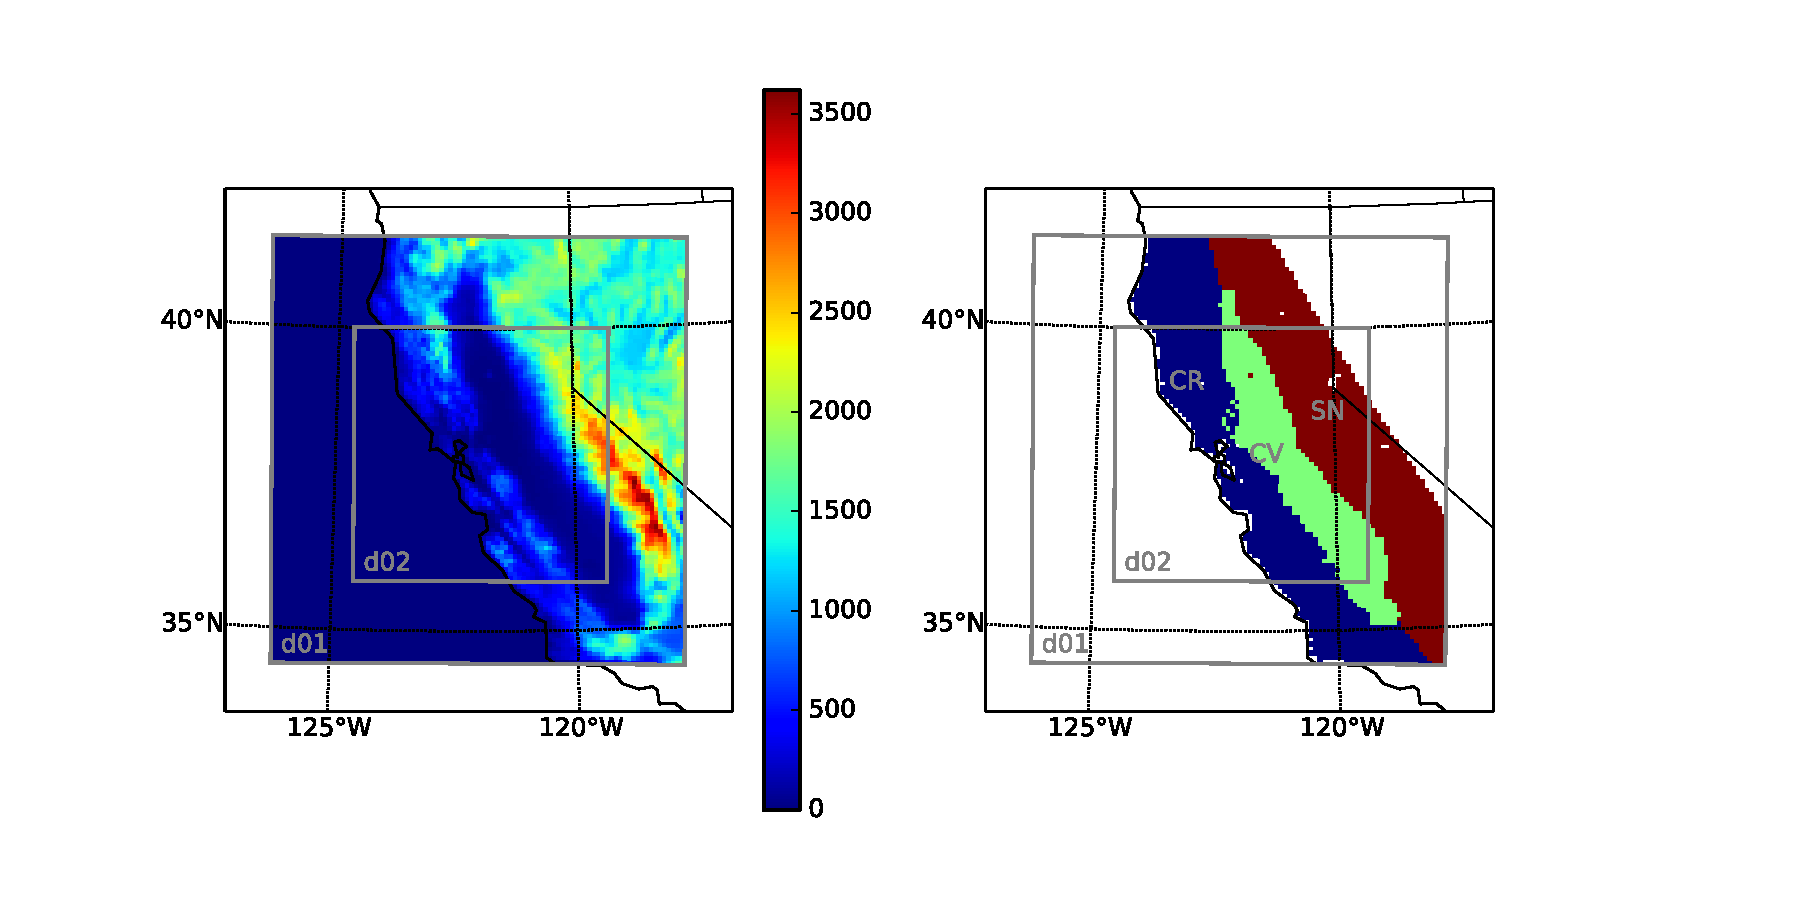
\includegraphics[width=1\textwidth]{ch3-wind/img/domain_map.pdf}
\caption{WRF model domains, showing (a) topographic height in m, and (b) the Coast Range (CR), Central Valley (CV), and Sierra Nevada (SN) regions for soil moisture tests. d01 refers to the outer model domain, and d02 refers to the inner domain.}
\label{fig:windSol_domainmap}
\end{figure}

\begin{table}
\begin{tabular}{ l c c c c c c c }
\hline
Domain & $\Delta x$ (km) & $\Delta y$ (km) & $nx$ & $ny$ & $nz$ & $\Delta t$ (s) & USGS data res \\ \hline
d01 & 8.1 & 8.1 & 96 & 99 & 45 & 45 & 2 min\\
d02 & 2.7 & 2.7 & 175 & 175 & 45 & 15 & 2 min\\
\hline
\end{tabular}
\caption{Model domains. d01 refers to the outer domain, and d02 refers to the inner domain.}
\label{table:windSol_domains}
\end{table}

The atmospheric model is coupled to the Noah land surface model with USGS land use and soil classifications.  The observed distributions of land use and soil types are used, as are the default vegetation water-use parameters for each land use type, in order to simulate as closely as possible the real present day sensitivity of Solano winds to soil moisture.  Uncertainties associated with errors in the model representation of water movement in the subsurface and plant water use are addressed in the Discussion. 

The ACM2 PBL scheme is used, following the recommendations of Marjanovic \textit{et al.} [2014] for a locally forced simple terrain case in California; this PBL scheme includes both local (small-scale turbulent) and nonlocal (large convective plume) vertical transport, and can thus simulate both stable and unstable conditions [Pleim, \textit{2007}].  The model is forced at the lateral boundaries with NCEP Eta 212 grid (40 km) operational analysis [NCEP, 1998].  Other parameterization schemes and settings are listed in Table \ref{table:windSol_paramschemes}.  Model variables are output every 30 minutes.

\begin{table}
\begin{tabular}{l l}
\hline
Scheme & Setting \\ \hline
WRF version & 3.6 \\
Grid nesting & two-way \\
Lateral boundary conditions & NCEP Eta analysis \\
Soil levels & 4 \\
Land use and soil categories & USGS \\
Land surface model & Noah \\
Surface layer & MM5 Monin-Obukhov \\
Planetary Boundary Layer (PBL) & ACM2 \\
Microphysics & WSM 3-class simple ice \\
Longwave radiation & RRTM \\
Shortwave radiation & Dudhia \\
Cumulus & Kain-Fritsch (new Eta) \\
Turbulence closure & Horizontal Smagorinzky first order \\
Momentum advection & 5th order horizontal, 3rd order vertical \\
Scalar advection & Positive definite \\
Lateral boundary & 5 grid points \\
\hline
\end{tabular}
\caption{WRF parameterization options.  All options, except the PBL scheme, are the default settings in WRF.  See Skamarock \textit{et al.} [2008] for description of schemes.}
\label{table:windSol_paramschemes}
\end{table}

All experiments are run for the period 2009-06-26 00:00 UTC to 2009-07-11 00:00 UTC, and the first 32 hours are discarded as model spin-up.  This period was chosen for several reasons: (1) it contains a range of synoptic conditions (weak background wind June 27-July 5, and strong background wind July 6-11), (2) turbine-level wind speeds in this region are highest in the spring and summer [Zhong \textit{et al.}, 2004; Mansbach, 2010], and (3) the sensitivity to soil moisture is expected to be strongest in the warm season when radiation incident to the land surface is greatest, because changes in the relative partitioning between evapotranspiration and sensible heat flux have the largest absolute magnitude then.

\subsection{Soil moisture experiments}

The model experiments are listed in Table \ref{table:windSol_runlist}.  In the first set of experiments, we test the sensitivity of Solano winds to soil moisture in different large-scale regions of California.  In cases dryCR, dryCV, and drySN, the background volumetric soil moisture (model variable SMOIS, m$^3$ water/m$^3$ total volume) is set to 0.25, and the soil moisture of the test region (respectively, the Coast Range, Central Valley, and Sierra Nevada, shown in Figure \ref{fig:windSol_domainmap}b) is set to 0.1.  These test cases are compared with a control case where all land has soil moisture of 0.25.  In cases wetCR, wetCV, and wetSN, the background soil moisture is set to 0.1, and the soil moisture of the test region is set to 0.25.  These test cases are compared with a control case where all land has soil moisture of 0.1.

The next set of experiments tests how the Solano wind response scales with soil moisture in the Central Valley, with a normal-to-wet background in the Coast Range and Sierra Nevada.  In cases CVXX (where XX is a numeric value), the Coast Range and Sierra Nevada regions' soil moisture is set to 0.2, and the Central Valley soil moisture is set to the value specified by XX.  These test cases are compared with a control case where all land has soil moisture of 0.2.
%In cases CVXXdry, the Coast Range and Sierra Nevada regions' soil moisture is set to 0.1, and the Central Valley soil moisture again is specified by XX.

In all cases, the soil moisture is set to the prescribed values at the model start time (2009-06-26 00:00 UTC) and is reset to the prescribed value each day at 08:00 UTC (midnight Pacific Standard Time); the soil moisture evolves according to the land surface model each day between resets.  The change in soil moisture between resets is small (up to 0.02 m$^3$/m$^3$ in the regional average when soils are wet and much less when soils are dry; Figure \ref{fig:windSol_forcings}, panels 2-4).

\begin{figure}[here]
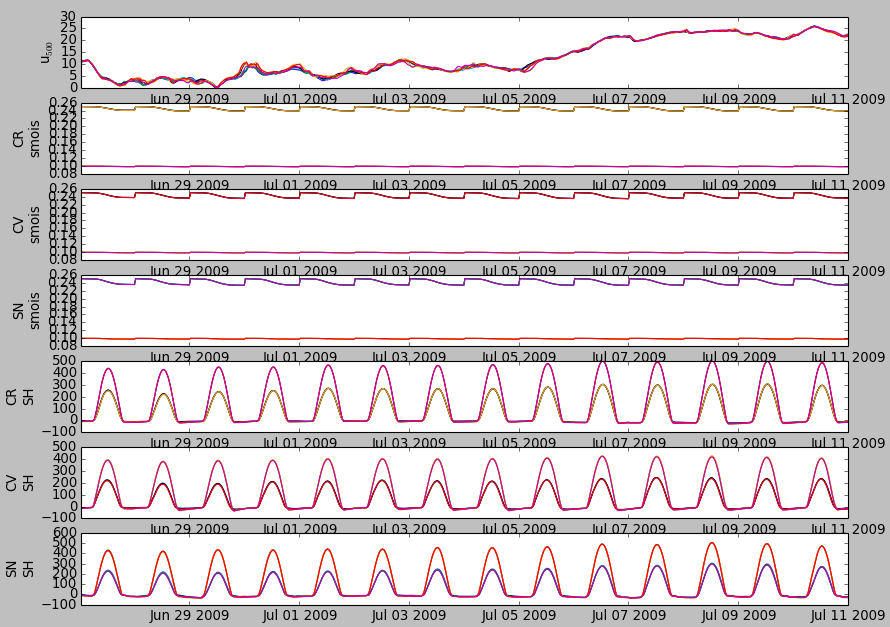
\includegraphics[width=1\textwidth]{ch3-wind/img/forcings_combo_good.png}
\caption{Model forcing for all of the regional perturbation cases.  \textbf{I NEED ADVICE ON HOW TO DISPLAY THIS INFORMATION MORE CLEARLY AND/OR CONCISELY. Obviously, I need a legend for which color means which run.}  Top panel: wind speed over Solano at 500 hPa.  Panels 2-4: average soil moisture in the top soil layer for the CR region (panel 2), the CV region (panel 3), and the SN region (panel 4).  Panels 5-7: average surface sensible heat flux for the CR region (panel 5), the CV region (panel 6), and the SN region (panel 7).}
\label{fig:windSol_forcings}
\end{figure}

\begin{table}
\begin{tabular}{l l l l}
\hline
Run name & Background SMOIS & Perturbed SMOIS region & Perturbed SMOIS value \\
\hline
CA-0.1 & 0.1 & none & n/a \\
CA-0.2 & 0.2 & none & n/a \\
CA-0.25 & 0.25 & none & n/a \\
dryCR & 0.25 & Coast Range & 0.1 \\
dryCV & 0.25 & Central Valley & 0.1 \\
drySN & 0.25 & Sierra Nevada & 0.1 \\
wetCR & 0.1 & Coast Range & 0.25 \\
wetCV & 0.1 & Central Valley & 0.25 \\
wetSN & 0.1 & Sierra Nevada & 0.25 \\
CV0.05 & 0.2 & Central Valley & 0.05 \\
CV0.1 & 0.2 & Central Valley & 0.1 \\
CV0.15 & 0.2 & Central Valley & 0.15 \\
CV0.25 & 0.2 & Central Valley & 0.25 \\
CV0.3 & 0.2 & Central Valley & 0.3 \\
CV0.35 & 0.2 & Central Valley & 0.35 \\
%CV0.05dry & 0.1 & Central Valley & 0.05 \\
%CV0.15dry & 0.1 & Central Valley & 0.15 \\
%CV0.2dry & 0.1 & Central Valley & 0.2 \\
%CV0.25dry & 0.1 & Central Valley & 0.25 \\
%CV0.3dry & 0.1 & Central Valley & 0.3 \\
%CV0.35dry & 0.1 & Central Valley & 0.35 \\
\hline
\end{tabular}
\caption{Model experiments}
\label{table:windSol_runlist}
\end{table}

%\end{document}